\documentclass{article}
\usepackage[utf8]{inputenc}

\usepackage{natbib}
\usepackage{graphicx}

\usepackage[slovene]{babel}
\usepackage{amsmath}
\usepackage{amsfonts}
\usepackage{amssymb}

\usepackage[T1]{fontenc}
\usepackage{listingsutf8}
\lstset{literate={č}{{\v c}}1 {š}{{\v s}}1 {ž}{{\v z}}1}

\usepackage{caption}
\usepackage{subcaption}

\title{Praktično delo III}
\author{Lovro Habjan}
\date{\today}

\begin{document}

\maketitle

\section{Uvod}

Problem trgovskega potnika je NP-poln problem, kjer iščemo najkrajši obhod vseh
mest, tako da vsako obiščemo le enkrat in se na koncu vrnemo v
začetno. Implementirali smo tri algoritme za metričnega trgovskega potnika. Zanj
velja, da za povezave med mesti velja trikotniška neenakost. Algoritme in
generiranje nalog smo implementirali v programskem jeziku \textit{python} s
pomočjo knjižnice \textit{networkx}.


\section{Generiranje instanc problema MTSP}

Instance problema za metričnega trgovskega potnika smo generirali tako, da smo v
ravnini $\mathbb{R}^2$ naključno izbirali točke. Vsaka točka je predstavljala
neko vozlišče, teže povezav med vozlišči pa smo izračunali kot razdaljo med
točkami. Na ta način smo zadostili trikotniški neenakosti. Grafe, ki smo jih
generirali, so bili polno povezani.


\section{Algoritmi}

Implementirali smo tri algoritme za metričnega trgovskega potnika:
\begin{enumerate}
\item Požrešen algoritem: Implementirali smo algoritem s hevristiko najbližjega
  soseda. Začnemo v nekem vozlišču in nato vedno izberemo njegovega najbližjega
  soseda, ki še ni obiskan. Na koncu se iz zadnjega mesta vrnemo v prvotno.
\item 2-aproksimacijski algoritem: Pri tem algoritmu najprej zgradimo minimalno
  vpeto drevo, nato pa po drevesu naredimo obhod v globino. Podvojena vozlišča
  odstranimo iz cikla.
\item Christofidesov algoritem: Najprej zgradimo minimalno vpeto drevo. Iz njega
  izberemo vozlišča z liho stopnjo povezav in poiščemo največje popolno ujemanje
  na grafu, ki ga ta vozlišča inducirajo. Drevo in povezave z ujemanja združimo
  skupaj in izvedemo Eulerjev obhod. Iz njega odstranimo podvojena vozlišča.
\end{enumerate}

\section{Empirično ovrednotenje}

Algoritme smo testirali tako, da smo za različne velikosti naključno generiranih
grafov merili čas izvajanja in primerjali rešitve med seboj. Generirali smo
grafe velikosti $|V| = [10, 310]$. Uporabili smo dva različna nabora grafov; pri
prvem smo točke generirali s koordinatami $10 \times 10$, pri drugem pa z
večjimi $1000 \times 1000$, kar nam je dalo grafe z manjšimi in z večjimi
razdaljami. Za vsak nov $n$ smo generirali 10 poljubnih grafov.

Najprej si poglejmo primere z manjšimi razdaljami. Slika~\ref{fig:time10}
prikazuje povprečen čas izvajanja glede na velikost grafa. Vidimo, da sta
požrešni in 2-aproksimacijski algoritem zelo hitra in da njuna časovna
zahtevnost zelo počasi narašča. Nasprotno velja za Christofidesov algoritem,
kjer se čas izvajanja z našo implementacijo hitro
poveča. Slika~\ref{fig:rezultati10} prikazuje, kako dobre so rešitve algoritmov
pri različnih $n$. Vidimo, da z naraščanjem $n$ Christofidesov algoritem vrača
najboljše rezultate. Presenetil nas je požrešen algoritem, saj se je v skoraj
vseh primerih izkazal za bolj natančnega kot 2-aproksimacijski algoritem.

V primeru večjih razdalj vidimo podobne rezultate. Slika~\ref{fig:time1000}
prikazuje povprečen čas izvajanja pri grafih z večjih razdaljah in vidimo, da
razlik s prejšnjim naborom grafov skoraj ni. Slika~\ref{fig:rezultati1000}
prikazuje kvaliteto rešitev in vidimo, da so tudi rezultati primerljivi.

\begin{figure}
	\centering
	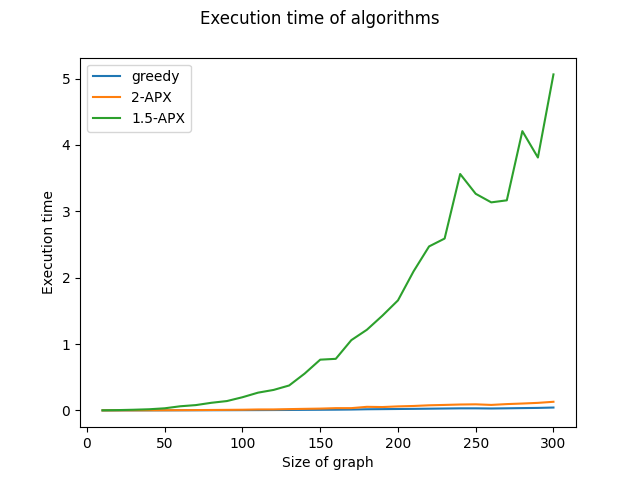
\includegraphics[width = 0.8\textwidth]{figs/time10.png}
	\caption{Čas izvajanja pri manjših razdaljah}
	\label{fig:time10}
\end{figure}

\begin{figure}
	\begin{subfigure}{0.5\textwidth}
		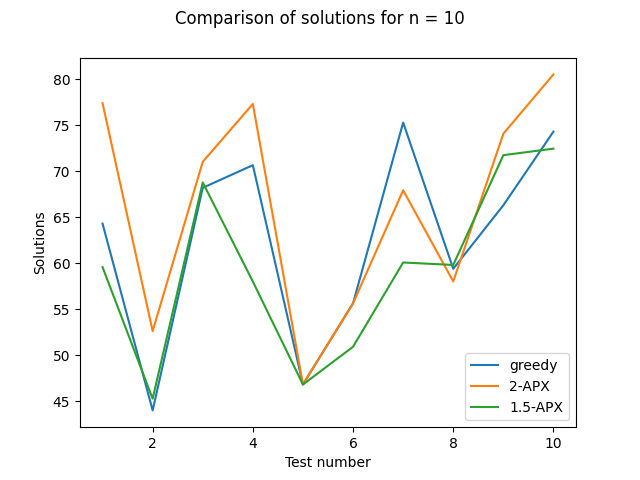
\includegraphics[width=\textwidth]{figs/results10-1.png}
		\caption{$n = 10$}
		\label{fig:rezultat10-1}
	\end{subfigure}
	\begin{subfigure}{0.5\textwidth}
		\centering
		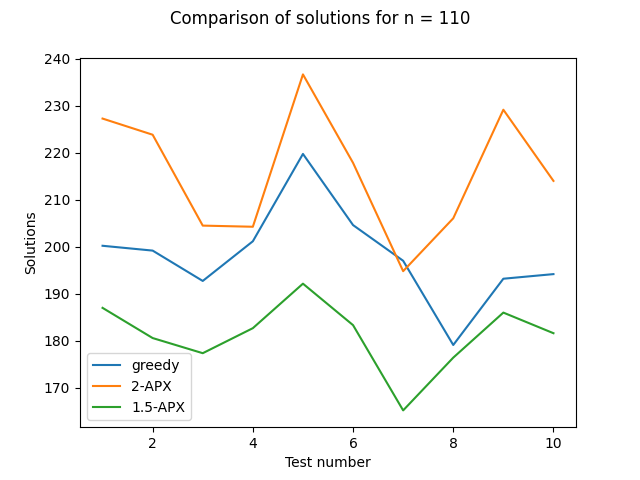
\includegraphics[width=\textwidth]{figs/results10-2.png}
		\caption{$n = 110$}
		\label{fig:rezultat10-2}
	\end{subfigure}
	\newline
	\begin{subfigure}{0.5\textwidth}
		\centering
		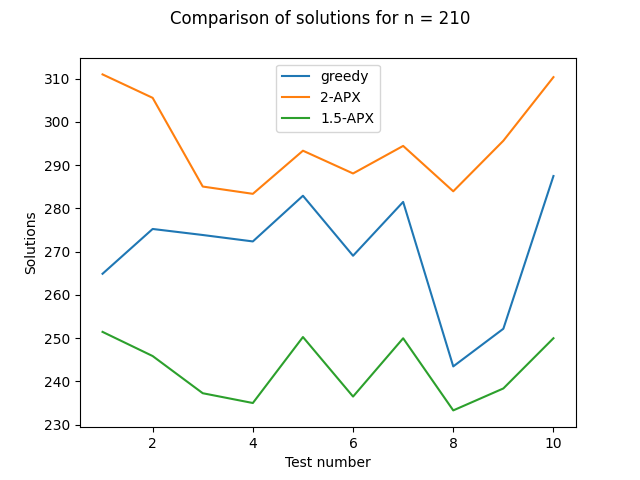
\includegraphics[width=\textwidth]{figs/results10-3.png}
		\caption{$n = 210$}
		\label{fig:rezultat10-3}
	\end{subfigure}
	\begin{subfigure}{0.5\textwidth}
		\centering
		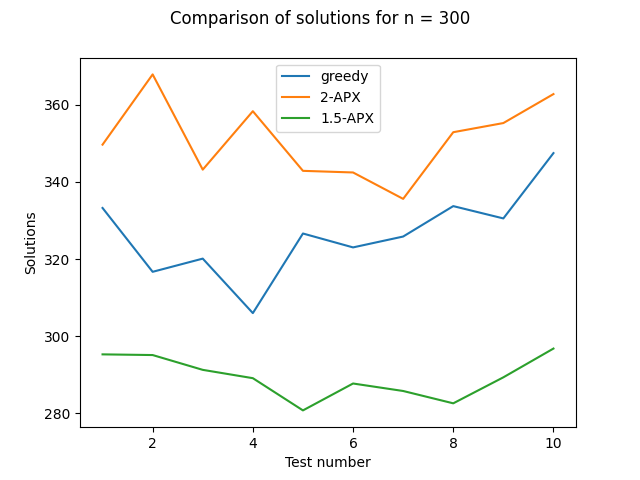
\includegraphics[width=\textwidth]{figs/results10-4.png}
		\caption{$n = 300$}
		\label{fig:rezultat10-4}
	\end{subfigure}
	\caption{Primerjava algoritmov pri različnih $n = |V|$ za majhne razdalje}
	\label{fig:rezultati10}
\end{figure}

\begin{figure}
	\centering
	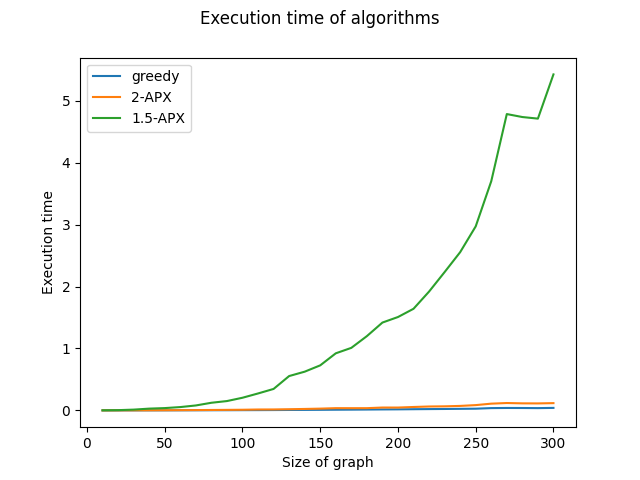
\includegraphics[width = 0.8\textwidth]{figs/time1000.png}
	\caption{Čas izvajanja pri večjih razdaljah}
	\label{fig:time1000}
\end{figure}

\begin{figure}
	\begin{subfigure}{0.5\textwidth}
		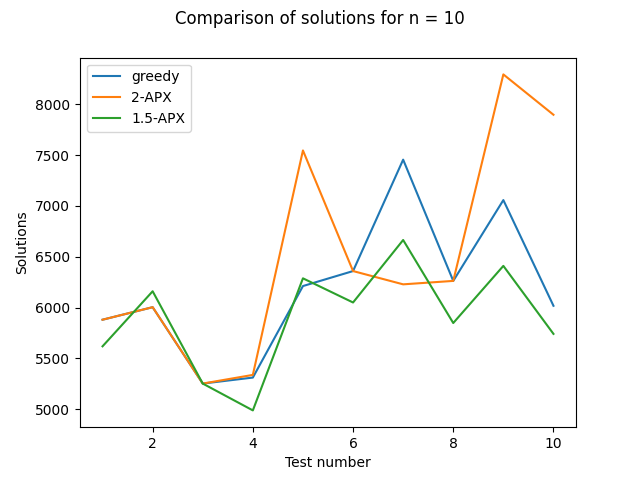
\includegraphics[width=\textwidth]{figs/results1000-1.png}
		\caption{$n = 10$}
		\label{fig:rezultat1000-1}
	\end{subfigure}
	\begin{subfigure}{0.5\textwidth}
		\centering
		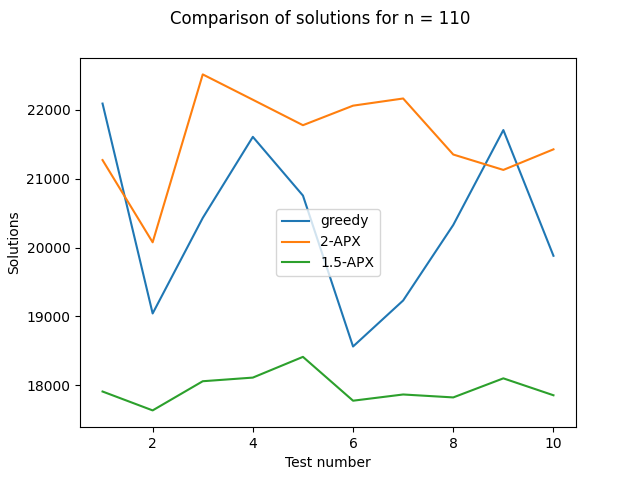
\includegraphics[width=\textwidth]{figs/results1000-2.png}
		\caption{$n = 110$}
		\label{fig:rezultat1000-2}
	\end{subfigure}
	\newline
	\begin{subfigure}{0.5\textwidth}
		\centering
		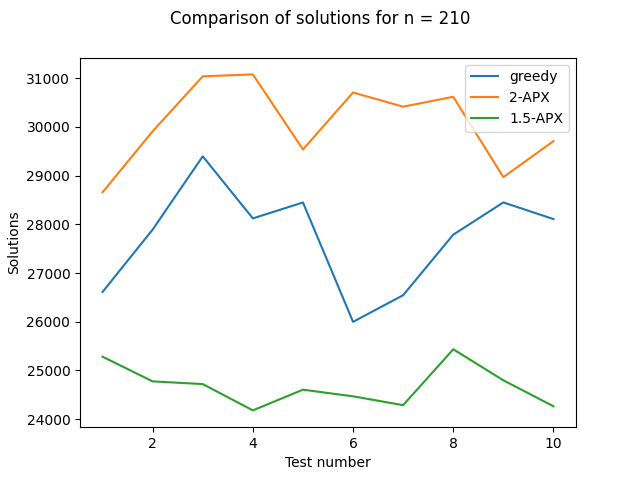
\includegraphics[width=\textwidth]{figs/results1000-3.png}
		\caption{$n = 210$}
		\label{fig:rezultat1000-3}
	\end{subfigure}
	\begin{subfigure}{0.5\textwidth}
		\centering
		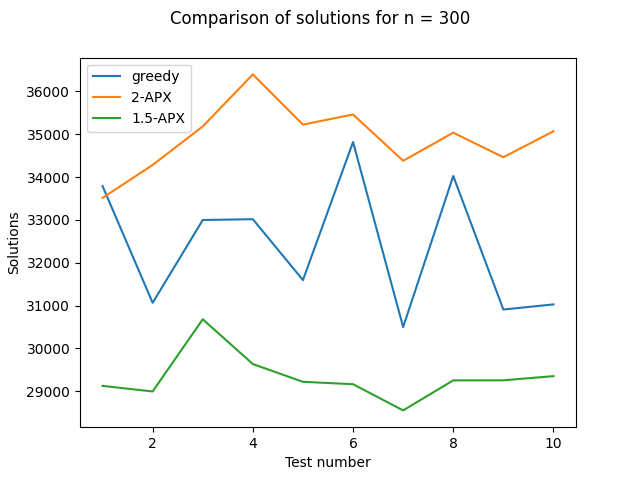
\includegraphics[width=\textwidth]{figs/results1000-4.png}
		\caption{$n = 300$}
		\label{fig:rezultat1000-4}
	\end{subfigure}
	\caption{Primerjava algoritmov pri različnih $n = |V|$ za večje razdalje}
	\label{fig:rezultati1000}
\end{figure}


\section{Zaključek}

Z empiričnim ovrednotenjem algoritmov za problem metričnega trgovskega potnika
smo pokazali, da je najbolj natančen algoritem Christofidesov, ki je
1,5-aproksimacijski, a je tudi najpočasnejši. Kljub naivni implementaciji se
požrešni algoritem izakže za dobrega, saj je v skoraj vseh primerih bil boljši
od 2-aproksimacijskega.

\end{document}